% XCircuit output "dram_cell.tex" for LaTeX input from dram_cell.eps
\def\putbox#1#2#3#4{\makebox[0in][l]{\makebox[#1][l]{}\raisebox{\baselineskip}[0in][0in]{\raisebox{#2}[0in][0in]{\scalebox{#3}{#4}}}}}
\def\rightbox#1{\makebox[0in][r]{#1}}
\def\centbox#1{\makebox[0in]{#1}}
\def\topbox#1{\raisebox{-0.60\baselineskip}[0in][0in]{#1}}
\def\midbox#1{\raisebox{-0.20\baselineskip}[0in][0in]{#1}}
\begin{center}
   \scalebox{0.8}{
   \normalsize
   \parbox{2.8125in}{
   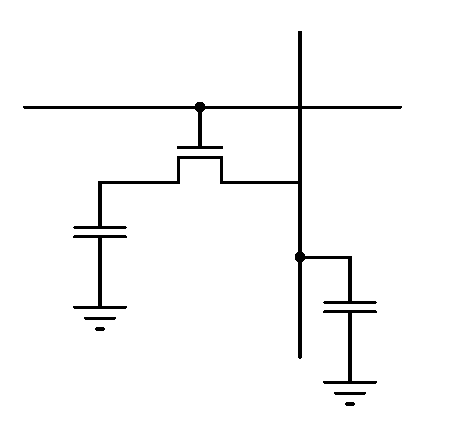
\includegraphics[scale=1]{memorie/dram_cell.eps}\\
   % translate x=640 y=348 scale 0.38
   \putbox{1.97in}{2.45in}{1.20}{$BL$}%
   \putbox{0.14in}{2.20in}{1.20}{$WL$}%
   \putbox{0.81in}{1.12in}{1.20}{$C_b$}%
   \putbox{2.47in}{0.70in}{1.20}{$C_L$}%
   } % close 'parbox'
   } % close 'scalebox'
   \vspace{-\baselineskip} % this is not necessary, but looks better
\end{center}
